% Ergebnisse und Analyse Diagramme.tex

\newcommand{\MergesortMaxArrayVerdoppelnMesswerte}{%
    \addplot[blue, mark=*] coordinates {
            (25000000,3017372600)
            (50000000,6315632400)
            (100000000,12777405700)
            (200000000,27203738300)
            (400000000,56441153000)
        };
    \addlegendentry{Mergesort}
}

\newcommand{\QuicksortMaxArrayVerdoppelnMesswerte}{%
    \addplot[green, mark=*] coordinates {
            (25000000,1528071600)
            (50000000,3248990900)
            (100000000,6653966800)
            (200000000,13778762100)
            (400000000,29074726600)
        };
    \addlegendentry{Quicksort}
}


\newcommand{\MergesortMiniArrayVerdoppeln}{%
    \addplot[blue, mark=*] coordinates {
            (1,1000)
            (2,1300)
            (4,3100)
            (8,3200)
            (16,3500)
            (100,8700)
            (1000,97700)
            (2000,191700)
            (4000,354400)
        };
    \addlegendentry{Quicksort}
}

\newcommand{\QuicksortMiniArrayVerdoppeln}{%
    \addplot[green, mark=*] coordinates {
            (1,2700)
            (2,2800)
            (4,3100)
            (8,3800)
            (16,3300)
            (100,3000)
            (1000,34900)
            (2000,73100)
            (4000,148500)
        };
    \addlegendentry{Quicksort}
}

\newcommand{\GrundlegendeLaufzeitenAbhaengigVonDerArraygroesseDiagrammA}{%
    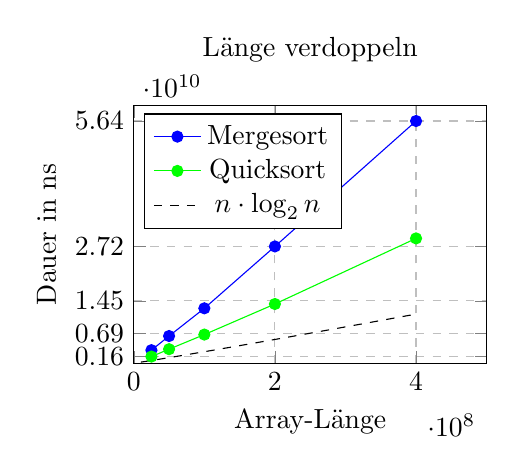
\begin{tikzpicture}
        \begin{axis}[
                title style={yshift=1.5ex},
                width=0.5\textwidth,
                height=0.4\textwidth,
                xlabel={Array-Länge},
                ylabel={Dauer in ns},
                title={Länge verdoppeln},
                xmin=0, xmax=5 * 10^8,
                ymin=0*10^6, ymax=6*10^10,
                grid=both,
                grid style=dashed,
                legend pos=north west,
                ytick={1609541400,6854920900,14495472700,27203738300,56441153000},
                % xtick={2^21,2^23,2^24,2^25},
                % xticklabels={$2^{21}$, $2^{23}$, $2^{24}$, $2^{25}$},
                % scaled x ticks=false,
                % scaled y ticks=false,
            ]
            \MergesortMaxArrayVerdoppelnMesswerte
            \QuicksortMaxArrayVerdoppelnMesswerte
            % n*log2(n)
            \addplot[black, dashed,domain=1e7:4e8, samples=100] {x*log2(x)};
            \addlegendentry{$n \cdot \log_2 n$}
            % % n
            % \addplot[red, dashed,domain=1e7:4e8, samples=100] {x};
            % \addlegendentry{$n$}
            % % log2(n)
            % \addplot[green, domain=1e7:4e8, samples=100] {log2(x)};
            % \addlegendentry{$\log_2 n$}
        \end{axis}
    \end{tikzpicture}%
}

\newcommand{\GrundlegendeLaufzeitenAbhaengigVonDerArraygroesseDiagrammB}{%
    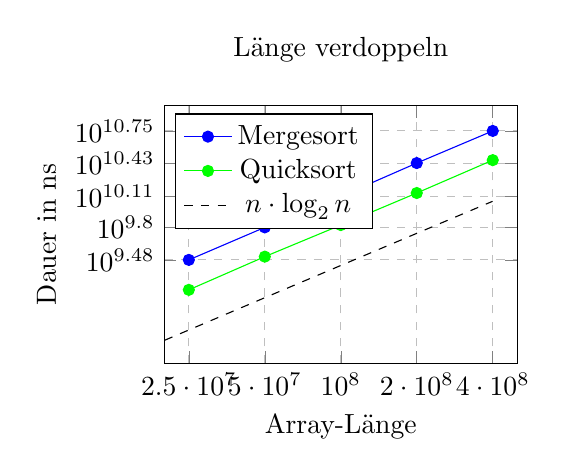
\begin{tikzpicture}
        \begin{axis}[
                title style={yshift=1.5ex},
                width=0.5\textwidth,
                height=0.4\textwidth,
                xlabel={Array-Länge},
                ylabel={Dauer in ns},
                title={Länge verdoppeln},
                xmin=2*10^7, xmax=5 * 10^8,
                ymin=0*10^6, ymax=1*10^11,
                grid=both,
                grid style=dashed,
                legend pos=north west,
                xmode=log,
                log basis x=10,
                xtick=data,
                xticklabels={$2.5\cdot10^7$, $5\cdot10^7$, $10^8$, $2\cdot10^8$, $4\cdot10^8$},
                ymode=log,
                log basis y=10,
                ytick=data,
                % xtick={2^21,2^23,2^24,2^25},
                % xticklabels={$2^{21}$, $2^{23}$, $2^{24}$, $2^{25}$},
                % scaled x ticks=false,
                % scaled y ticks=false,
            ]
            \MergesortMaxArrayVerdoppelnMesswerte
            \QuicksortMaxArrayVerdoppelnMesswerte
            % n*log2(n)
            \addplot[black, dashed,domain=1e7:4e8, samples=100] {x*log2(x)};
            \addlegendentry{$n \cdot \log_2 n$}
        \end{axis}
    \end{tikzpicture}%
}

\newcommand{\GrundlegendeLaufzeitenAbhaengigVonDerArraygroesseDiagrammC}{%
    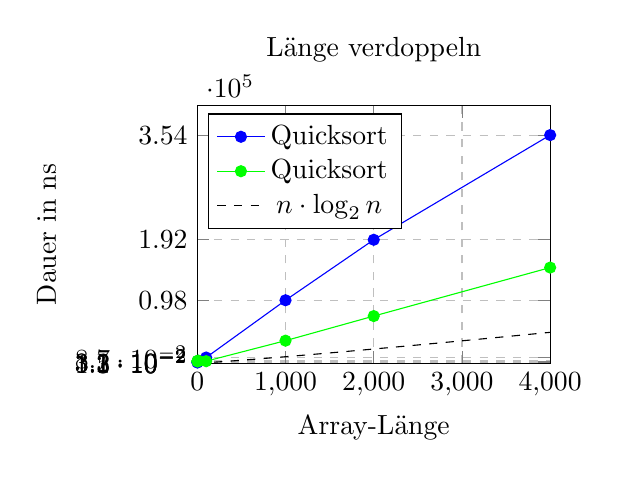
\begin{tikzpicture}
        \begin{axis}[
                title style={yshift=1.5ex},
                width=0.5\textwidth,
                height=0.4\textwidth,
                xlabel={Array-Länge},
                ylabel={Dauer in ns},
                title={Länge verdoppeln},
                xmin=0, xmax=4000,
                ymin=0, ymax=4*10^5,
                grid=both,
                grid style=dashed,
                legend pos=north west,
                ytick=data,,
                % xtick={2^21,2^23,2^24,2^25},
                % xticklabels={$2^{21}$, $2^{23}$, $2^{24}$, $2^{25}$},
                % scaled x ticks=false,
                % scaled y ticks=false,
            ]
            \MergesortMiniArrayVerdoppeln
            \QuicksortMiniArrayVerdoppeln
            % n*log2(n)
            \addplot[black, dashed,domain=1:4000, samples=100] {x*log2(x)};
            \addlegendentry{$n \cdot \log_2 n$}
            % % n
            % \addplot[red, dashed,domain=1e7:4e8, samples=100] {x};
            % \addlegendentry{$n$}
            % % log2(n)
            % \addplot[green, domain=1e7:4e8, samples=100] {log2(x)};
            % \addlegendentry{$\log_2 n$}
        \end{axis}
    \end{tikzpicture}%
}

\newcommand{\GrundlegendeLaufzeitenAbhaengigVonDerArraygroesseDiagrammD}{%
    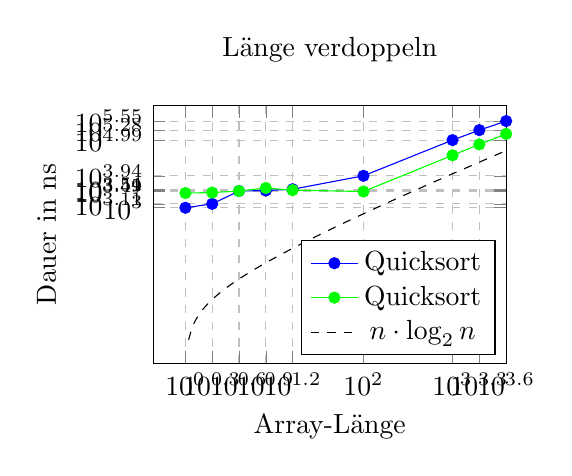
\begin{tikzpicture}
        \begin{axis}[
                title style={yshift=1.5ex},
                width=0.5\textwidth,
                height=0.4\textwidth,
                xlabel={Array-Länge},
                ylabel={Dauer in ns},
                title={Länge verdoppeln},
                xmin=0, xmax=4000,
                ymin=0, ymax=1*10^6,
                grid=both,
                grid style=dashed,
                legend pos=south east,
                xmode=log,
                log basis x=10,
                xtick=data,
                % xticklabels={$2.5\cdot10^7$, $5\cdot10^7$, $10^8$, $2\cdot10^8$, $4\cdot10^8$},
                ymode=log,
                log basis y=10,
                ytick=data,
                % xtick={2^21,2^23,2^24,2^25},
                % xticklabels={$2^{21}$, $2^{23}$, $2^{24}$, $2^{25}$},
                % scaled x ticks=false,
                % scaled y ticks=false,
            ]
            \MergesortMiniArrayVerdoppeln
            \QuicksortMiniArrayVerdoppeln
            % n*log2(n)
            \addplot[black, dashed,domain=1:4000, samples=100] {x*log2(x)};
            \addlegendentry{$n \cdot \log_2 n$}
        \end{axis}
    \end{tikzpicture}%
}
